%  \documentclass[DIV=12, a4]{scrartcl}
%\documentclass[12pt, a5]{scrartcl}

% \documentclass[a4paper]{report}
% \usepackage[
% % fancytheorems, 
% noindent, 
% %spacingfix, 
% %noheader
% ]{vanilla}


\documentclass[a4paper]{scrreprt}
\usepackage[
fancytheorems, 
noindent, 
% %spacingfix, 
% %noheader,
fancyproofs
]{adam} 

\usepackage{tikz}
\usepackage{siunitx}
\usepackage{asymptote}
\usetikzlibrary{calc,patterns,angles,quotes,snakes}


% \usepackage{subfig}

% \setcounter{chapter}{-1}

\title{Dynamics and Relativity}
% \subtitle{Adam Kelly}
\author{Adam Kelly}
% \date{Michaelmas 2020}
\date{\today}

\begin{document}

\maketitle

\begin{abstract}
	
	% \vspace{2\baselineskip}
	% {\color{red} None of the notes here have been reviewed at all, and are just exactly what was taken down live in the lectures. I would turn around now and come back in a few days, when I have gone back, cleaned things up, fixed explanations and added some structure.}
	% \vspace{5\baselineskip}

	This set of notes is a work-in-progress account of the course `Dynamics and Relativity', originally lectured by Prof Peter Haynes in Lent 2020 at Cambridge. These notes are not a transcription of the lectures, but they do roughly follow what was lectured (in content and in structure).

	These notes are my own view of what was taught, and should be somewhat of a superset of what was actually taught. I frequently provide different explanations, proofs, examples, and so on in areas where I feel they are helpful. Because of this, this work is likely to contain errors, which you may assume are my own. If you spot any or have any other feedback, I can be contacted at \href{mailto:ak2316@cam.ac.uk}{ak2316@cam.ac.uk}.


	% {\color{red} Notes written upto lecture 6.}
	% During the creation of this document, I consulted a number of other books and resources. All of these are listed in the bibliography. 

\end{abstract}

\tableofcontents

% \clearpage
% \chapter{Introduction}

% Most of the phenomena in everyday lives involve randomness. What we try to do in probability is model this randomness in a mathematical way. It's likely that you have studied some probability before, but the difference in the treatment here is that we will try to be somewhat more rigerous.

% We will define the notion of a probability space, where `our experiments take place'. Then we will discuss discrete and continuous random variables. 
% In the discrete setting, we will find that there is no real subtleties, and we can be quite rigorous. In the continuous setting however we will have to take some things for granted (but rigour will return in the Part II course).

% \begin{quote}
% 	\emph{``Probability theory has a right and a left hand. On the right is the rigorous foundational work using the tools of measure theory. The left hand `thinks probabilistically,' reduces problems to gambling situations, coin-tossing, motions of a physical particle.''}
% \end{quote}

% In this course, we will need both hands.


\chapter{Newtonian Dynamics -- Basic Concepts}

A central aspect of this course is Newtonian dynamics. In this chapter we will develop some of the ideas and definitions needed to discuss this in detail.


\section{Particles}

When dealing with Newtonian dynamics, we will often use and refer to \emph{particles}, as a way of describing phenomina.

\begin{definition}[Particle]
	A \vocab{particle} is an object of negligible size. It has some mass $m > 0$, and can also have other properties such as (perhaps) an electric charge $q$.
\end{definition}

A particle is completely described by a \vocab{position vector}, usually denoted $\vv{r}(t)$ or $\vv{x}(t)$, with respect to some origin $O$. The cartesian coordinates of $\vv{r}$ are $(x, y, z)$, where
$$
\vv{r} = x \vv{i} + y \vv{j} + z \vv{k},
$$
with $\vv{i}, \vv{j}, \vv{k}$ being orthonormal basis vectors.

\begin{center}


	\tikzset{every picture/.style={line width=0.75pt}} %set default line width to 0.75pt        

	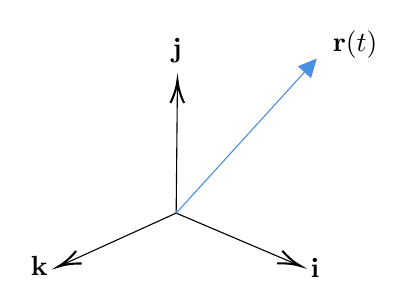
\begin{tikzpicture}[x=0.75pt,y=0.75pt,yscale=-1,xscale=1]
	%uncomment if require: \path (0,300); %set diagram left start at 0, and has height of 300
	
	%Straight Lines [id:da3885177182468236] 
	\draw    (306.66,120.4) -- (307.27,58.42) ;
	\draw [shift={(307.29,56.42)}, rotate = 450.56] [color={rgb, 255:red, 0; green, 0; blue, 0 }  ][line width=0.75]    (10.93,-3.29) .. controls (6.95,-1.4) and (3.31,-0.3) .. (0,0) .. controls (3.31,0.3) and (6.95,1.4) .. (10.93,3.29)   ;
	%Straight Lines [id:da43094715547088136] 
	\draw    (306.66,120.4) -- (364.76,145.12) ;
	\draw [shift={(366.6,145.9)}, rotate = 203.05] [color={rgb, 255:red, 0; green, 0; blue, 0 }  ][line width=0.75]    (10.93,-3.29) .. controls (6.95,-1.4) and (3.31,-0.3) .. (0,0) .. controls (3.31,0.3) and (6.95,1.4) .. (10.93,3.29)   ;
	%Straight Lines [id:da42613880767302603] 
	\draw    (306.66,120.4) -- (251.68,145.37) ;
	\draw [shift={(249.86,146.19)}, rotate = 335.58000000000004] [color={rgb, 255:red, 0; green, 0; blue, 0 }  ][line width=0.75]    (10.93,-3.29) .. controls (6.95,-1.4) and (3.31,-0.3) .. (0,0) .. controls (3.31,0.3) and (6.95,1.4) .. (10.93,3.29)   ;
	%Straight Lines [id:da8673951558603283] 
	\draw [color={rgb, 255:red, 74; green, 144; blue, 226 }  ,draw opacity=1 ]   (306.66,120.4) -- (372.43,48.15) ;
	\draw [shift={(374.45,45.93)}, rotate = 492.31] [fill={rgb, 255:red, 74; green, 144; blue, 226 }  ,fill opacity=1 ][line width=0.08]  [draw opacity=0] (8.93,-4.29) -- (0,0) -- (8.93,4.29) -- cycle    ;
	
	% Text Node
	\draw (370.19,140.92) node [anchor=north west][inner sep=0.75pt]    {$\mathbf{i}$};
	% Text Node
	\draw (303.48,34.86) node [anchor=north west][inner sep=0.75pt]    {$\mathbf{j}$};
	% Text Node
	\draw (235.39,139.92) node [anchor=north west][inner sep=0.75pt]    {$\mathbf{k}$};
	% Text Node
	\draw (380.9,31.33) node [anchor=north west][inner sep=0.75pt]    {$\mathbf{r}( t)$};
	
	
	\end{tikzpicture}
	
\end{center}

The choice of coordinate axes defines a \vocab{frame of reference} $S$.

Of course, we will be considering particles that are moving, so we will define the velocity, momentum and acceleration of the particle.

\begin{definition}[Velocity]
	The \vocab{velocity} of a particle is
	$
	\vv{u}(t) = \frac{\mathrm{d}}{\mathrm{d}t} \vv{r}(t) = \dot{\vv{r}},
	$
	and is tangent to the path (or trajectory) of the particle.
\end{definition}

\begin{definition}[Momentum]
	The \vocab{momentum} of a particle is
	$
	\vv{p} = m \vv{u} = m \dot{\vv{r}},
	$
	where $m$ is the mass of the particle.
\end{definition}

\begin{definition}[Acceleration]
	The \vocab{acceleration} of the particle is $\dot{\vv{u}} = \ddot{\vv{r}} = \frac{\mathrm{d}^2}{\mathrm{d}t^2} \vv{r}(t)$.
\end{definition}

\section{Newton's Laws of Motion}

We can now write down Newton's three laws of motion, which govern the motion of particles. All of these statements about particles can be extended to finite bodies (which are composed of many particles).

\begin{law*}[Newton's First Law/Galileo's Law of Inertia]
There exist inertial frames of reference in which a particle remains at rest or moves at constant velocity unless it is acted on by a force.
\end{law*}

\begin{law*}[Newton's Second Law]
	In an inertial frame the rate of change of momentum of a particle is equal to the force acting on it.
\end{law*}

\begin{law*}[Newton's Third Law]
To every action there is an equal and opposite reaction. That is, forces excreted between two particles are equal in magnitude and opposite in direction.
\end{law*}

We will see how these are used in the coming sections.

\section{Inertial Frames \& Galilean Transformations}

We met inertial frames in the previous section. In this section we will look at what inertial frames are and how they relate to each other.

\begin{definition}[Inertial Frame]
	In an \vocab{inertial frame}, the acceleration of a particle is zero if the force is zero. That is
	$$
	\ddot{\vv{r}} = \vv{0} \iff \vv{F} = \vv{0}.
	$$
\end{definition}

Inertial frames are not unique. For example, if $S$ is an inertial frame then any other frame $S'$ moving with constant velocity relative to $S$ is also an inertial frame. 
\begin{center}
	

\tikzset{every picture/.style={line width=0.75pt}} %set default line width to 0.75pt        

\begin{tikzpicture}[x=0.75pt,y=0.75pt,yscale=-1,xscale=1]
%uncomment if require: \path (0,300); %set diagram left start at 0, and has height of 300

%Straight Lines [id:da6554316462419089] 
\draw    (234,60) -- (234,140) ;
%Straight Lines [id:da4345590790645234] 
\draw    (304,180) -- (234,140) ;
%Straight Lines [id:da32274818064920674] 
\draw    (234,140) -- (174,180) ;
%Straight Lines [id:da67079104059405] 
\draw    (472,60) -- (472,140) ;
%Straight Lines [id:da9093648966502794] 
\draw    (542,180) -- (472,140) ;
%Straight Lines [id:da322772395178044] 
\draw    (472,140) -- (412,180) ;
%Straight Lines [id:da573637511432038] 
\draw [color={rgb, 255:red, 74; green, 144; blue, 226 }  ,draw opacity=1 ]   (472,80) -- (527.16,99.02) ;
\draw [shift={(530,100)}, rotate = 199.03] [fill={rgb, 255:red, 74; green, 144; blue, 226 }  ,fill opacity=1 ][line width=0.08]  [draw opacity=0] (8.93,-4.29) -- (0,0) -- (8.93,4.29) -- cycle    ;

% Text Node
\draw (306,181) node [anchor=north west][inner sep=0.75pt]    {$x$};
% Text Node
\draw (231,42) node [anchor=north west][inner sep=0.75pt]    {$y$};
% Text Node
\draw (163,179) node [anchor=north west][inner sep=0.75pt]    {$z$};
% Text Node
\draw (216,127) node [anchor=north west][inner sep=0.75pt]    {$O$};
% Text Node
\draw (228,205) node [anchor=north west][inner sep=0.75pt]    {$( t)$};
% Text Node
\draw (181,52) node [anchor=north west][inner sep=0.75pt]  [color={rgb, 255:red, 208; green, 2; blue, 27 }  ,opacity=1 ]  {$S$};
% Text Node
\draw (542,181) node [anchor=north west][inner sep=0.75pt]    {$x'$};
% Text Node
\draw (467,42) node [anchor=north west][inner sep=0.75pt]    {$y'$};
% Text Node
\draw (399,179) node [anchor=north west][inner sep=0.75pt]    {$z'$};
% Text Node
\draw (452,127) node [anchor=north west][inner sep=0.75pt]    {$O'$};
% Text Node
\draw (466,205) node [anchor=north west][inner sep=0.75pt]    {$( t')$};
% Text Node
\draw (419,52) node [anchor=north west][inner sep=0.75pt]  [color={rgb, 255:red, 208; green, 2; blue, 27 }  ,opacity=1 ]  {$S'$};
% Text Node
\draw (531,92) node [anchor=north west][inner sep=0.75pt]  [color={rgb, 255:red, 74; green, 144; blue, 226 }  ,opacity=1 ]  {$\vv{v}$};


\end{tikzpicture}

\end{center}

In the example above, it is easy to relate the coordinate systems in each system.
\begin{align*}
	\vv{r}' = \vv{r} - \vv{v}t,
\end{align*}
where $\vv{v}$ is the velocity of $S'$ relative to $S$. This transformation is called a \vocab{boost}.

For a particle with position vector $\vv{r}(t)$ in $S$ and $\vv{r}'(t')$ in $S'$, we can relate the velocity and acceleration as measured in $S$ and $S'$. Let the velocity be $\vv{u} = \dot{\vv{r}}(t)$ in $S$ and the acceleration be $\vv{a} = \ddot{\vv{r}}(t)$ in $S$. Then these relate to the corresponding quantities in $S'$ by
$$
\vv{u}' = \vv{u} - \vv{v}, \quad \quad \vv{a}' = \vv{a}.
$$

Boosts aren't the only transformations of frames that preserve inertial frames.

\begin{definition}[Galilean Frames]
	A \vocab{Galilean transformation} preserves inertial frames.
	The set of all Galilean transformations forms the \vocab{Galilean group}.
\end{definition}

Galilean frames combine boosts with some combination of the following:
\begin{itemize}
	\item Translations of space, $\vv{r}' = \vv{r} - \vv{r}_0$ where $\vv{r}_0$ is constant.
	\item Translations of time, $t' = t - t_0$ where $t_0$ is constant.
	\item Rotations and reflections in space, $\vv{r}' = R \vv{r}$ where $R$ is an orthogonal matrix.
\end{itemize}
This set generates the Galilean group.

For any Galilean transformation we have
$$
\ddot{\vv{r}} = \vv{0} \iff \ddot{\vv{r}'} = \vv{0},
$$
that is, $S$ inertial if and only if $S'$ is inertial.

\begin{law*}[Galilean Relativity]
	The principle of Galilean relativity is that the laws of Newtonian physics are the same in all inertial frames.
\end{law*}

This principle tells us that the the laws of physics are the same at any point in space, at any point in time, in whatever direction I face, and at whatever constant velocity I move with. Thus any set of equations which describe Newtonian physics must have these properties, known as \vocab{Galilean invariance}. 

Note that the measurement of velocity is then not absolute, but measurement of acceleration is.

\section{Newton's Second Law and Equations of Motion}

We previously stated Newton's second law, it says that for a particle subject to a force $\vv{F}$, the momentum $\vv{p}$ satisfies
$$
\frac{
	\mathrm{d} \vv{p}
}{\mathrm{d} t} = \vv{F},
$$
where the momentum $\vv{p} = m \vv{u} = m \dot{\vv{r}}$. 

For now, we will assume that $m$, the mass of the particle, is constant (we will return to the variable mass case later in the course). That gives us
$$
m \frac{\mathrm{d} \vv{u}}{\mathrm{d} t} = m \ddot{\vv{r}} = \vv{F}.
$$
In this way, we can describe mass as a measure of the `reluctance to accelerate', the inertia of the particle.

If $\vv{F}$ is specified as a function of $\vv{r}, \dot{\vv{r}}$ and $t$, $\vv{F}(\vv{r}, \dot{\vv{r}}, t)$, then we have a second order differential equation for $\vv{r}$. To solve this completely, we would need to prove the initial position $\vv{r}(t_0)$ and the initial velocity $\dot{\vv{r}}(T_0)$, then we get a unique solution. The path/trajectory of the particle is then determined (at all future and past times).

To get further, we will need to consider some possible forms of $vv{F}$.

\section{Examples of Forces}

\subsection{Gravitational Force}

Consider two particles with position vectors $\vv{r}_1$ and $\vv{r}_2$ and masses $m_1$ and $m_2$. Then we can describe the gravitational forces between them as follows.


\begin{law*}[Newton's Gravitation Law]
	\vocab{Newton's law of gravitation} states that the force of gravity between the particles is
	$$
	\vv{F}_1 = \frac{G m_1 m_2 (\vv{r}_1 - \vv{r}_2)}{|\vv{r}_1 - \vv{r}_2|^3} = -\vv{F}_2,
	$$
	where $G$ is the gravitational constant.
\end{law*}

Note that $\vv{F}_1 = \vv{F}_2$ is proportional to $|\vv{r}_1 - \vv{r}_2|^{-1}$, so we call this law an \vocab{inverse square law}.

We will explore the details of gravitational forces later on in the course.

\subsection{Electromagnetic Forces}

Consider a particle with electric charge $q$, in the presence of an electric field $\vv{E}(\vv{r}, t)$ and a magnetic field $\vv{B}(\vv{r}, t)$. Then we can describe the electromagnetic force as follows.

\begin{law*}[Lorentz Force Law]
	The electromagnetic force on the particle is
	$$
	\vv{F}(\vv{r}, \dot{\vv{r}}, t) = q(\vv{E}(\vv{r}, t) + \dot{\vv{r}} \times \vv{B}(\vv{r}, t)).
	$$
\end{law*}

\begin{example}
	Consider the case of $\vv{E} = \vv{0}$ and $\vv{B}$ being a constant vector.

	We can then use Newton's second law to get the equations of motion,
	$$
	m \ddot{\vv{r}} = q \dot{\vv{r}} \times \vv{B}.
	$$
	We will choose axes such that $\vv{B} = B \hat{vv{z}}$. Hence
	$$
	m \ddot{z} = 0 \implies z = z_0 + ut,
	$$
	for constants $z_0$ and $u$. We also get
	\begin{align*}
		m \ddot{x} &= qB \dot{y}\\
		m \ddot{y} &= -qB \dot{x}.
	\end{align*}
	Then defining $\omega  = qB/m$, we get the solution
	\begin{align*}
		x &= x_0 - \alpha \cos (\omega(t - t_0)),\\
		y &= y_0 + \alpha \sin(\omega(t - t_0)),
	\end{align*}
	where $x_0, x_0, t_0$ and $\alpha$ are constants determined by the initial conditions.

	Geometrically, the motion of the particle is made up of circular motion in $x, y$ and constant velocity in $z$, which is helical motion in the direction of the magnetic field. The motion is also clockwise from the direction of $\vv{B}$.
\end{example}

\chapter{Dimensional Analysis}

\section{Units and Dimensional Quantities}

Many of the problems we think about in dynamics involve three basic dimensional quantities: 
\begin{itemize}
	\item $L$ -- length,
	\item $M$ -- mass,
	\item $T$ -- time.
\end{itemize}
The dimensions of some quantity $[x]$\footnote{It will be convenient throughout this section to use the notation $[x]$ to denote the dimensions of $x$, using the shorthand of $L$, $M$ and $T$ as described above.} can be expressed in terms of $L, M, T$.
For example, $[\text{density}] = M \cdot L^{-3}$ and $[\text{force}] = M \cdot L \cdot T^{-2}$.

There are some rules that apply to the dimensions of a quantity. Specifically, we only allow power law functions of $L, M, T$. 
For example, if $X$ was some dimensional quantity, then $e^X = 1 + X + X^2/2 + \cdots$ wouldn't make any sense because we would be using different dimensions and units.

We usually use the standard SI set of units for $L, M$ and $T$. We have \si{m} (meters) for length $L$, \si{kg} (kilograms) for mass $M$ and \si{s} (seconds) for time $T$. Many other physical quantities can be formed out of these basic units. 

\begin{example}[Newton's Gravitational Constant]
	Consider the gravitational constant $G$ appearing in Newton's Law of Gravitation, described previously.

	We had the force $F = \frac{Gm_1 m_2}{r^2}$ for masses $m_1, m_2$ and length $r$, Thus we have
$$
	G = \frac{F \cdot r^2}{m_1 m_2} \implies [G] = \frac{M \cdot L \cdot L^2}{T^2 \cdot M \cdot M} = \frac{L^3}{M \cdot T^2}.
$$
So the natural units for $G$ will be \si{m^3 .kg^{-1}. s^{-2}}. Indeed, if we choose those units we would find that $G = \SI{6.67e-11}{m^3 .kg^{-1}. s^{-2}}$.
\end{example}

The general principle is that dynamical/physical equations must work for \emph{any} consistent choice of units.

\section{Scaling}

Suppose that we had some dimensional quantity $Y$, depending on some other set of dimensional quantities $X_1, X_2, \dots, X_n$. Let the dimensions be $[Y] = L^a M^b T^c$, and $[X_i] = L^{a_i} M^{b_i} T^{c_i}$ for $i \in \{1, \dots, n\}$. 

If $n \leq 3$, then $Y = C \cdot X_1^{p_1} X_2^{p_2} X_3^{p_3}$, and $p_1, p_2, p_3$ can be determined by balancing dimensions:
$$
L^a M^b T^c = (L^{a_1} M^{b_1} T^{c_1})^{p_1} \cdots
$$
hence we have $a = a_1 p_1 + a_2 p_2 + a_3 p_3$, and similarly for $b$ and $c$. Then we have three unknowns for $p_1, p_2, p_3$ if the dimensions $X_1, X_2, X_3$ are independent.

If $n > 3$, then the property of dimensional independence cannot extend for $X_1, X_2, \dots$, but we can choose $X_1$, $X_2$ and $X_3$ that are (without loss of generality) dimensionally independent and $n - 3$ dimensionless quantities $\lambda_1 = \frac{X_4}{X_1^{q_{11}} X_2^{q_{12}} X_3^{q_{13}}}$ and so on, where $q_{mn}$ are chosen to balance the dimensions.

Then $Y = X_1^{p_1} X_2^{p_2} X_3^{p_3} \cdot C(\lambda_1, \dots, \lambda_{n - 3})$. This is `Bridgeman's theorem'. 

\begin{example}[Period of a Pendulum]
	Consider a simple pendulum as shown below.
	\begin{center}
		

% Pattern Info
 
\tikzset{
	pattern size/.store in=\mcSize, 
	pattern size = 5pt,
	pattern thickness/.store in=\mcThickness, 
	pattern thickness = 0.3pt,
	pattern radius/.store in=\mcRadius, 
	pattern radius = 1pt}
	\makeatletter
	\pgfutil@ifundefined{pgf@pattern@name@_9n48vb0tk}{
	\pgfdeclarepatternformonly[\mcThickness,\mcSize]{_9n48vb0tk}
	{\pgfqpoint{0pt}{0pt}}
	{\pgfpoint{\mcSize+\mcThickness}{\mcSize+\mcThickness}}
	{\pgfpoint{\mcSize}{\mcSize}}
	{
	\pgfsetcolor{\tikz@pattern@color}
	\pgfsetlinewidth{\mcThickness}
	\pgfpathmoveto{\pgfqpoint{0pt}{0pt}}
	\pgfpathlineto{\pgfpoint{\mcSize+\mcThickness}{\mcSize+\mcThickness}}
	\pgfusepath{stroke}
	}}
	\makeatother
	\tikzset{every picture/.style={line width=0.75pt}} %set default line width to 0.75pt        
	
	\begin{tikzpicture}[x=0.75pt,y=0.75pt,yscale=-1,xscale=1]
	%uncomment if require: \path (0,300); %set diagram left start at 0, and has height of 300
	
	%Shape: Rectangle [id:dp9368435998112152] 
	\draw  [draw opacity=0][pattern=_9n48vb0tk,pattern size=6pt,pattern thickness=0.75pt,pattern radius=0pt, pattern color={rgb, 255:red, 0; green, 0; blue, 0}] (60,90) -- (250,90) -- (250,100) -- (60,100) -- cycle ;
	%Straight Lines [id:da27141557633818303] 
	\draw    (60,100) -- (250,100) ;
	%Straight Lines [id:da1403199835183353] 
	\draw  [dash pattern={on 4.5pt off 4.5pt}]  (150,100) -- (150,200) ;
	%Straight Lines [id:da09553429066707841] 
	\draw    (150,100) -- (230,190) ;
	%Shape: Circle [id:dp1277453731851712] 
	\draw  [fill={rgb, 255:red, 0; green, 0; blue, 0 }  ,fill opacity=1 ] (220,190) .. controls (220,184.48) and (224.48,180) .. (230,180) .. controls (235.52,180) and (240,184.48) .. (240,190) .. controls (240,195.52) and (235.52,200) .. (230,200) .. controls (224.48,200) and (220,195.52) .. (220,190) -- cycle ;
	%Straight Lines [id:da8816498309072955] 
	\draw    (150,210) -- (230,210) ;
	\draw [shift={(230,210)}, rotate = 180] [color={rgb, 255:red, 0; green, 0; blue, 0 }  ][line width=0.75]    (0,5.59) -- (0,-5.59)(10.93,-3.29) .. controls (6.95,-1.4) and (3.31,-0.3) .. (0,0) .. controls (3.31,0.3) and (6.95,1.4) .. (10.93,3.29)   ;
	\draw [shift={(150,210)}, rotate = 0] [color={rgb, 255:red, 0; green, 0; blue, 0 }  ][line width=0.75]    (0,5.59) -- (0,-5.59)(10.93,-3.29) .. controls (6.95,-1.4) and (3.31,-0.3) .. (0,0) .. controls (3.31,0.3) and (6.95,1.4) .. (10.93,3.29)   ;
	%Straight Lines [id:da6422563646516952] 
	\draw    (230,190) -- (230,250) ;
	\draw [shift={(230,250)}, rotate = 270] [color={rgb, 255:red, 0; green, 0; blue, 0 }  ][line width=0.75]    (17.64,-4.9) .. controls (13.66,-2.3) and (10.02,-0.67) .. (6.71,0) .. controls (10.02,0.67) and (13.66,2.3) .. (17.64,4.9)(10.93,-4.9) .. controls (6.95,-2.3) and (3.31,-0.67) .. (0,0) .. controls (3.31,0.67) and (6.95,2.3) .. (10.93,4.9)   ;
	
	% Text Node
	\draw (197,132) node [anchor=north west][inner sep=0.75pt]    {$l$};
	% Text Node
	\draw (187,212) node [anchor=north west][inner sep=0.75pt]    {$d$};
	% Text Node
	\draw (242,172) node [anchor=north west][inner sep=0.75pt]    {$( m)$};
	% Text Node
	\draw (237,242) node [anchor=north west][inner sep=0.75pt]    {$g$};
	
	
	\end{tikzpicture}
	
	\end{center}
	We want to know how the period of oscillation $P$ depends on the quantities $m, l, d$ and $g$. Here, we have $Y$ being the period and $X_1, X_2, X_3$ and $X_4$ being the four quantities $m, l, d$ and $g$. So let's think about the dimensions.
	\begin{align*}
		[P] &= T \\
		[m] &= M\\
		[g] &= L \cdot T^{-2} \quad \quad \text{(gravity)} \\
		[l] &= L\\
		[d] &= L
	\end{align*}
	Now we form the one dimensionless group by taking the ratio $d/l$, writing
	$$
	P = f\left(\frac{d}{l}\right) m^{p_1} l^{p_2} g^{p_3},
	$$
	which is the dimensional statement
	$$
	T = M^{p_1} L^{p_2} \left(\frac{L}{T^2}\right)^{p_3}.
	$$
	Balancing dimensions, we have that $M: p_1 = 0$, $L: p_2 + p_3 = 0$, and $T: 1 = -2p_3$. Solving these we get $p_1 = 0, p_2 = 1/2$ and $p_3 = -1/2$. Thus we get
	$$
	P = f(d/l) l^{1/2} g^{-1/2}.
	$$
	There is of course a lot of freedom in this formula (as we haven't really considered the physical situation), but it does contain useful information. For example, if $d \mapsto 2d$ and $l \mapsto 2l$, then $p \mapsto \sqrt{2}p$. But if $d \mapsto 2d$ and $l \mapsto l$, then we couldn't say much because it depends on the precise form of $f$. 
\end{example}

\chapter{Forces}

\section{Force and Potential Energy in 1 Spacial Dimension}

Consider a mass $m$ moving in a straight line with position $x(t)$.
Let's suppose we had some force that depends only on position $x$, and not velocity $\dot{x}$ or time $t$.
We will call the force $F(x)$, and define potential energy as follows.

\begin{definition}[Potential Energy]
	The \vocab{potential energy} $V(X)$ is given by $F(x) = -\frac{\dd V}{\dd x}$, so
	$$
	V(x) = - \int^x F(x') \; \dd x'.
	$$
\end{definition}

We know that the force satisfies newton's second law, $m \ddot{x} = - \frac{\dd V}{\dd x}$. We also define kinetic energy.

\begin{definition}[Kinetic Energy]
	The \vocab{kinetic energy} $T(\dot{x}) = \frac{1}{2} m\dot{x}^2$. In higher dimensions, this is generalized to $\frac{1}{2}, |\dot{\vv{x}}|^2$.
\end{definition}

Now, if we take the kinetic and potential energy we get an important invariant.

\begin{proposition}[Conservation of Energy]
	The total energy $E = T + V$ is conserved. That is, $\frac{\dd E}{\dd t} = 0$.
\end{proposition}
\begin{proof}
	Differentiating we have
	\begin{align*}
		\frac{\dd E}{\dd t} &= \frac{\dd}{\dd t} \left(\frac{1}{2} v \dot{x}^2 + V(x)\right) \\
		&= m \dot{x}\ddot{x} + \frac{\dd V}{\dd x} \dot{x} \\
		&= \dot{x} \left(m \ddot{x} + \frac{\dd V}{\dd x} \right) = 0,
	\end{align*}
	as required.
\end{proof}

Note that for conservation of $\frac{1}{2} m \dot{x}^2 + \Phi$, we require $\dot F = -\frac{\dd \Phi}{\dd t}$. In principle, $\Phi$ may depend on $x, \dot{x}$ and $t$. But usually it is the case that there is no such $\Phi$ if $F$ depends on $\dot{x}$ and/or $t$.

\begin{example}[Harmonic Oscillator]
	Consider a system where $F(x) = -k x$ (physical examples of such system is Hooke's law for an elastic string). Then
	$$
	V(x) = -\int^x (-kx') \; \dd x' = \frac{1}{2}k x^2,
	$$
	with an appropriate choice of arbitrary constant.
	We can then seek an explicit expression for $x(t).$ We know that $m \ddot{x} = -kx$, hence
	$$
x(t) = A \cos \omega t + B \sin \omega t,
	$$
	and
	$$
\dot{x} = - \omega A \sin \omega t + \omega B \cos \omega t,
$$
for suitable constants $A$ and $B$ and $\omega = (k/m)^{1/2}$.

We can then verify that energy is conserved. The total energy is $E = \frac{1}{2}m \dot{x}^2 + \frac{1}{2}kx^2 = \frac{1}{2}(-\omega A \sin \omega t + \omega B \cos \omega t)^2 m + \frac{1}{2}k (A \omega \sin \omega t + B 
\sin \omega t)^2 = \frac{1}{2}k(A^2 + B^2)$, which is a constant. 
\end{example}

Let's now think about more general potentials. In one dimension, conservation of energy gives useful information about the motion. 

We can think of conservation as the first integral of Newton's second law. If we have
$$
E = \frac{1}{2} m \dot{x}^2 + V(x) \quad \quad \text{constant},
$$
then
$$
\dot{x} = \pm\sqrt{\frac{2}{3}(E - V(X))},
$$
where $E$ is set by the initial conditions.
Hence
$$
\pm \int_{x_0}^{x} \frac{\dd x'}{\sqrt{\frac{2}{3}(E - V(X))}} = t - t_0
$$
with $x = x_0$ when $t = t_0$. We get an implicit solution for $x(t)$. Of course, there is a limit to how much can be taken analytically from this integral, but  
in principle (possibly numerically) this integral could be evaluated to find $x(t)$.

We can gain some qualitative insights from the conservation of energy.

\begin{example}
	Take $V(x) = \lambda(x^3 - 3 \beta^2 x)$ where $\lambda, \beta$ are positive constants.
	\begin{center}
		\begin{asy}
			unitsize(55);
			import graph;
			pair F(real x) {
				return (0.5*x, 0.5*0.3*(x^3 - 3*x));
			}
	
			path g = graph(F, -2.1, 2.1);
	
			draw(g, blue + linewidth(0.9pt));
	
			draw((0, -0.55) -- (0, 0.55), arrow=Arrow(TeXHead));
			draw((-1.3, 0) -- (1.3, 0), arrow=Arrow(TeXHead));

			label("$V(x)$", (1.6, 0.44415), blue);
		\end{asy}
	\end{center}
	We can wonder what happens if we release the particle from rest at $x=x_0$ for various choices of $x_0$. 

	The assumption of stating from rest implies that the total energy is $V(x_0)$. Then conservation of energy implies that $V(x) \leq V(x_0)$.

	If the left maxima is at $x = -\beta$ and the right minima is at $x = \beta$, then we can consider cases of the value of $x$. 

	If $x_0 < -\beta$, then the particle will keep moving to the left, going to $- \infty$. If $- \beta < x_0 < 2 \beta$, then the particle must stay confined to this region. If $x_0 > 2\beta$, then the particle will move to the left, will reach $x = -\beta$ and will then continue to $- \infty$.
	
	Some special cases are $x_0 = - \beta$, where the particle will stay at $-\beta$, and $x_0 = \beta$ where the particle will stay at $\beta$. Lastly, if $x_0 = 2 \beta$, then the particle will move to the left, and will come to rest at $x = - \beta$.
\end{example}

\end{document}
